
%----------------------------------------------------------------------------------------
%	CHAP Biomart
%----------------------------------------------------------------------------------------

\chapterimage{blue-chapter-head_4-reduced.pdf} % Chapter heading image
\chapter{Biomart}\label{chap:Biomart}
%upload images for examples
%invert description and itemize statement

% introduction
\section{Overview}
<<<<<<< HEAD
The BioMart project develops software and data services that are made available to the international scientific community. Users of MetaR can access data marts provided by BioMart, providing access to a wide range of research data . Similarly to EdgeR and Limma, BioMart support is provided in a MetaR language extension. This means that in order to access BioMart with MetaR, you first need to add the \textit{Biomart} language to the model where you create the analysis. To do so, you can press~\keys{\ctrl+L} and add language \textit{org\allowbreak.campagnelab\allowbreak.metar\allowbreak.biomart}. After adding the \textit{biomart} language to the model, you can create \texttt{query biomart} statements, described in the following sections. 

\section{The Biomart Statement}\index{query biomart statement},\index{Biomart}
The \texttt{query biomart} statement makes it possible to interactively specify which data should be retrieved from a mart (using attributes and filters). Data downloaded from Biomart will be stored in a new table. Figure~\ref{fig:NewBiomart} presents a newly created \texttt{query biomart} statement.
The \texttt{query biomart} statement has the following parameters.
\begin{itemize}
\item \texttt{database} This is the source database that will be queried to retrieve data.
\item \texttt{dataset} This is the dataset, inside the database that will provide data.
\item \texttt{attributes} These attributes describe which columns of data will be downloaded and stored in the result table.
\item \texttt{filters} These filters control which rows of data will be retrieved from the dataset.
=======
The BioMart project develops software and data services that are made available to the international scientific community. Users of MetaR can access data Marts provided by BioMart, providing access to a wide range of research data . Similarly to EdgeR and Limma, BioMart support is provided in a MetaR language extension. This means that in order to access BioMart with MetaR, you first need to add the Biomart language to the model where you create the analysis. To do so, you can press~\keys{\ctrl+L} and add language \textit{org\allowbreak.campagnelab\allowbreak.metar\allowbreak.biomart}. After adding the biomart language to the model, you can create \texttt{query biomart} statements, described in the following sections. 

\section{The Biomart Statement}
The \texttt{query biomart} statement makes it possible to interactively specify which data should be retrieved from a mart (using attributes and filters). Data downloaded from Biomart will be stored in a new table. Figure~\ref{fig:NewBiomart} presents a newly created Biomart statement.
The \texttt{query biomart} statement has the following parameters.
\begin{itemize}
\item database
\item dataset
\item attributes
\item filters
>>>>>>> 2df7b74af062bfb9bc71458f7cfc7b834b0d9370
\end{itemize} 

 \begin{figure}[h!tbp]
  \centering
  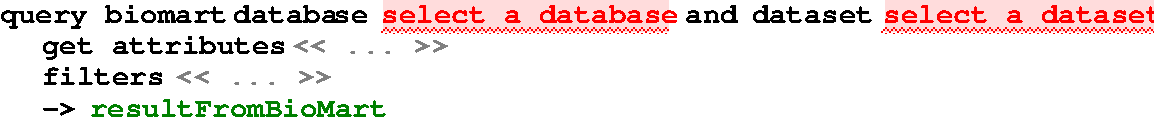
\includegraphics[width=\figWidthWide]{figures/NewBiomart.pdf}
\caption[New Query Biomart Statement.]{\textbf{New Query Biomart Statement.}}
\label{fig:NewBiomart}
\end{figure}


\paragraph{database}
<<<<<<< HEAD
The first time you create a \texttt{query biomart} statement in an Analysis, the statement will retrieve the list of available Biomart databases. To use one of these databases, use auto-completion over the \texttt{database} attribute (see  text \textit{select a database} in Figure~\ref{fig:NewBiomart}). Then, press \keys{\ctrl+\space} and select one database. Selecting the database will retrieve the set of datasets available in this database, which will become available with auto-completion.


 \paragraph{dataset} 
Once a database is selected, you need to choose a dataset inside this database. To choose one, press \keys{\ctrl+\space} to display all available datasets, on the text \textit{select a dataset}. You may use type keywords to identify the dataset of interest, similarly to other uses of auto-completion in MPS and MetaR. When a dataset is selected, you will need to configure its children:
\begin{itemize}

\item \texttt{attributes}, which will be the columns retrieved from the dataset that will populate the result table.
\item \texttt{filters}, which make it possible  to restrict the rows of data to retrieve.
\end{itemize}

\begin{remark}
In a few instances, you may find that a dataset cannot be associated with attributes or filters. In this case, in the auto completion menu for both attributes and filters will display the message \textit{"No available filter or attributes in this dataset"}. The selected dataset is no more available in Biomart. This means that this dataset, although available via the Biomart web service, cannot be used to retrieve data from the web service. You will need to select another database/dataset. 
\end{remark}

\paragraph{attributes}
Attributes are columns of the source dataset that will be written to the result table. Figure~\ref{fig:attributeBiomart} presents a new biomart attribute. An attribute has three parameters:
\begin{itemize}

\item \texttt{attribute}, a column you want to retrieve from the dataset and write to the result table. Press \keys{\ctrl+\space} to display the available column names.
\item \texttt{type}, the value type of the attribute. Choose a type for the column that will be created from the set: \texttt{boolean}, \texttt{numeric} or \texttt{string} (note that \texttt{string} is the default). To change the type, press \keys{\ctrl+\space}.
\item \texttt{column group}, an attribute can have a group such as "ID". The user can display the autocompletion menu by pressing \keys{\ctrl+\space}. Group must be defined in the Column Group Container to be added to columns created for the result table.
\end{itemize}

\begin{remark}
You must select at least one attribute before you can execute the \texttt{query biomart} Statement.
=======
The first time you will create the \texttt{query biomart} statement, you will automatically download the available Biomart databases. To choose one of them, go to the text \textit{select a database}. Then, press \keys{\ctrl+\space} to display all available databases. Select one of them by pressing \keys{\return}. 


 \paragraph{dataset} 
Once a database is selected, you need to choose a dataset. To choose one, press \keys{\ctrl+\space} to display all available datasets, on the text \textit{select a dataset}. Then, press \keys{\return}, to select your dataset. \newline
A dataset as two childrens:
\begin{itemize}
\item attributes, which will be the columns of your result table.
\item filters, which allow you to restrict your result table for some criteria.
\end{itemize}
\begin{remark}
Sometimes, a dataset cannot be associated with attributes or filters. In this case, in the auto completion menu for both attributes and filters will display the message \textit{"No available filter or attributes in this dataset"}. The selected dataset is no more available in Biomart. You must change your dataset or database. 
\end{remark}

\paragraph{attributes}
Attributes are columns of your result table. Figure~\ref{fig:attributeBiomart} presents a new biomart attribute. An attribute has three parameters:
\begin{itemize}
\item attribute, a column you want to retrieve on your result table. Press \keys{\ctrl+\space} to display the available column.
\item type, of  the attribute rows values. It exist three  types
boolean, numeric and string (\textit{ by default}). To change the type, press \keys{\ctrl+\space}.
\item column group, an attribute can have a group such as "ID". The user can display the autocompletion menu by pressing \keys{\ctrl+\space}. Group must be defined in the Column Group Container to be added to the result table.
\end{itemize}

\begin{remark}
You must select at least one column to run your query biomart Statement.
>>>>>>> 2df7b74af062bfb9bc71458f7cfc7b834b0d9370
\end{remark}

 \begin{figure}[h!tbp]
  \centering
  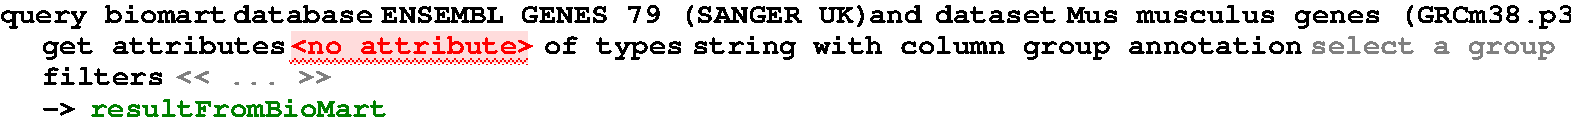
\includegraphics[width=\figWidthWide]{figures/BiomartAttribute.pdf}
<<<<<<< HEAD
\caption[Select an attribute in a biomart dataset.]{\textbf{Select an attribute in a biomart dataset.} An attribute contains any information you want to retrieve to populate the result table. Attributes have a name, a type and a column group annotation. The set of available attributes depends on the specific dataset selected.}
\label{fig:attributeBiomart}
\end{figure}
\paragraph{Filters}
Filters make it possible to restrict the result with some criteria. The types of filter available depend on the dataset selected in the statement. Figure~\ref{fig:BiomartFilter} presents a new biomart filter. There are four kinds of filters: 
\begin{itemize}

\item \texttt{boolean filters} select rows for which a value is either true or false. For example, if a gene has or does not have a Mirbase identitier.
\item \texttt{text filters} select rows which match some text in some attribute. The query will return only rows of the dataset that contain which match the text. For example, you can use a text filter to query rows that include a specific GO term.
\item \texttt{list filters} select rows that include an element among those of a finite list. Available list elements are determined by the mart dataset.  For example, a specific chromosome in a specie can be selected with a list filter.
\item \texttt{id list filters} select rows that contain a specific set of identifiers. These ids can be obtained either in a MetaR \texttt{SetOfIds} node, defined before the \texttt{query biomart} statement, or directly from an annotated table, where one column has an ID group.  

=======
\caption[Select an attribute in a biomart dataset.]{\textbf{Select an attribute in a biomart dataset.} An attribute contains any information you want to retrieve on your result table. It has a name, a type and a column group annotation. Attributes are related to a specific dataset.}
\label{fig:attributeBiomart}
\end{figure}
\paragraph{Filters}
Filters allow you to restrict your result for some criteria. this criteria are link directly to your dataset. Figure~\ref{fig:BiomartFilter} presents a new biomart filter. It exist four filter categories: 
\begin{itemize}
\item boolean, you want to retrieve or excluded only data which have an information. \textit{For example, if this gene has or has not a Mirbase ID.}
\item text, you have to enter a text in this area. the query will return only informations which match your text. \textit{For example  a specific GO term.}
\item list,  you need to choose a value from a define list. \textit{For example a specific chromosome in a specie.}
\item id list, you can restrict your results from a set of ids. This ids can come from a set of ids define before the statement, or directly from an annotated table with an (ID group).  
>>>>>>> 2df7b74af062bfb9bc71458f7cfc7b834b0d9370
\end{itemize}

 \begin{figure}[h!tbp]
  \centering
  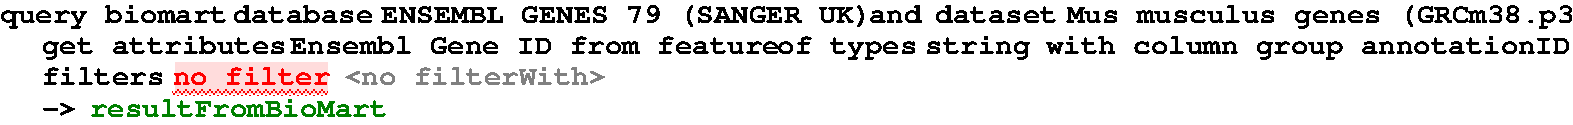
\includegraphics[width=\figWidthWide]{figures/BiomartFilter.pdf}
<<<<<<< HEAD
\caption[New Biomart Filter]{\textbf{New Biomart Filter.} A filter allow you to filter rows of the dataset according to some criterion. It exist four filters categories: boolean, text, list and id list. Filters are related to a specific dataset.}
=======
\caption[New Biomart Filter]{\textbf{New Biomart Filter.} A filter allow you to apply constraints to you results. It exist four filters categories: boolean, text, list and id list. Filters are related to a specific dataset.}
>>>>>>> 2df7b74af062bfb9bc71458f7cfc7b834b0d9370
\label{fig:BiomartFilter}
\end{figure}

\paragraph{table}
<<<<<<< HEAD
The future table where your result will be stored. Column annotations derived from the attribute type and column groups are displayed under the Inspector Tab (\inspectorTabIcon).
\section{Examples}
\subsection{Example 1}
Figure~\ref{fig:BiomartExample1} shows how to obtain a table from the Ensembl database and Human dataset. The result table "resultFromBiomart" contains two columns, the Ensembl Gene and Exon ID, where the first column is annotated as a group "ID". These results are filtered to exclude any gene that does not have a miRBase identifier.
=======
The future table where your result will be stored. Column annotation is display under the Inspector Tab (\inspectorTabIcon).
\section{Examples}
\subsection{Example 1}
Figure~\ref{fig:BiomartExample1} show how to obtain a table from the Ensembl database and Human dataset. The result table "resultFromBiomart" contains 2 columns, the Ensembl Gene and Exon ID, where the first column is annotated as a group "ID". This result are filters from a list of gene and which do not contains a Mirbase ID.
>>>>>>> 2df7b74af062bfb9bc71458f7cfc7b834b0d9370
 \begin{figure}[h!tbp]
  \centering
  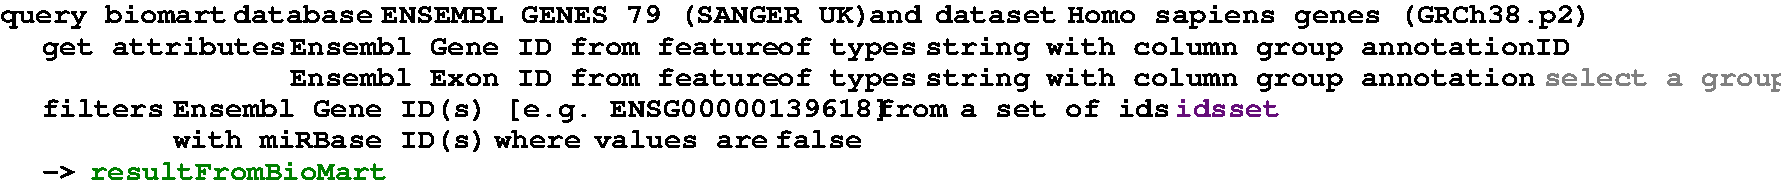
\includegraphics[width=\figWidthWide]{figures/BiomartExample1.pdf}
\caption[Biomart Example 1]{\textbf{ Biomart Example 1.}}
\label{fig:BiomartExample1}
\end{figure}

\subsection{Example 2}
<<<<<<< HEAD
Figure~\ref{fig:BiomartExample2} shows how to obtain a table from the \textit{Paramecium bibliography} database. The result table "resultFromBiomart" contains two columns, the PubMed ID and the abstract, where the publication year is equal or larger than 2000.
=======
Figure~\ref{fig:BiomartExample2} show how to obtain a table from the Paramecium bibliography. The result table "resultFromBiomart" contains 2 columns, the PubMed ID and the abstract, where the publication year is upper 2000.
>>>>>>> 2df7b74af062bfb9bc71458f7cfc7b834b0d9370
 \begin{figure}[h!tbp]
  \centering
  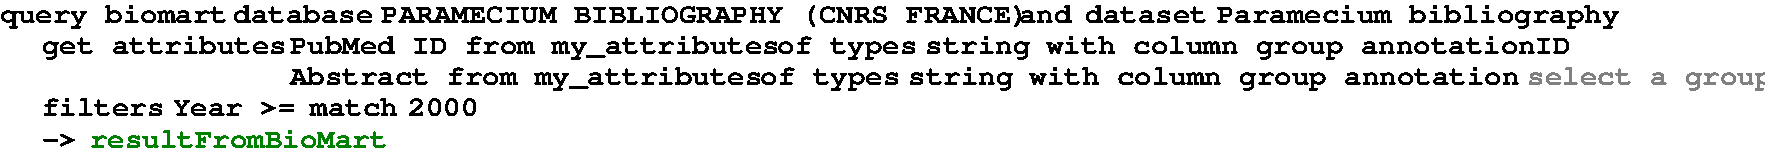
\includegraphics[width=\figWidthWide]{figures/BiomartExample2.pdf}
\caption[Biomart Example 2]{\textbf{ Biomart Example 2.}}
\label{fig:BiomartExample2}
\end{figure}
